\documentclass[11pt]{article}

\usepackage{fontspec}
\setmainfont{Palatino}
\setsansfont{Helvetica}
\setmonofont{Menlo}

\usepackage{kotex}
\setmainhangulfont{NanumMyeongjo}

\usepackage{amsmath, amssymb}
\usepackage[margin=1in]{geometry}
\usepackage{setspace}
\onehalfspacing
\usepackage{float}
\usepackage{graphicx}
\usepackage{booktabs}
\usepackage[authoryear]{natbib}
\setcitestyle{aysep={}}
\usepackage{xcolor}
\definecolor{blue}{RGB}{0,114,178}
\usepackage{hyperref}
\hypersetup{colorlinks, citecolor=blue, linkcolor=blue, urlcolor=blue}

\begin{document}
\setlength{\emergencystretch}{2em}

\title{Women's Bill Passage Across Electoral Pathways in the Korean National Assembly: A Reversal That Seniority Does Not Explain}
\author{KNA Research Agents (AI-generated)\thanks{AI-generation disclosure. This working paper was produced by an autonomous AI research-agent system without a human author of record. Version 2 was corrected by the orchestrating Claude session at the researcher's request. It is an experimental output and has not been peer-reviewed or independently fact-checked. See the statements preceding the bibliography.}\\[3pt]\textit{Experimental Output - kna-research-agents.com}}
\date{Version 2, 27 September 2026. Version 1, 1 April 2026.}
\maketitle
\thispagestyle{empty}

\noindent\rule{\linewidth}{0.6pt}

{\small
\setstretch{1.0}
\noindent\textbf{Correction notice.} Version 2, 2026-09-27. Corrected by the orchestrating Claude session at the researcher's request after an audit of the seniority coding. Every number in this version that comes from the data was produced by a rerun script or by the figure scripts, run on the kna v0.6.0 data that Version 1 used. Where a Version 1 value could not be reproduced even with the Version 1 coding, the notice says so and the paper reports the reproducible value. The changes are listed below, with each old value followed by its new value.

\begin{enumerate}
\setlength{\itemsep}{1pt}
\item \textbf{Seniority was miscoded.} Version 1 coded a lead sponsor as multi-term when the member file's \texttt{reelection} field did not read 초선. That field records each member's lifetime number of terms at the time the data were collected and takes the same value in every Assembly, so it is not seniority at an Assembly. A woman in her first term in the 21st Assembly who was re-elected in 2024 was coded as multi-term. Version 2 derives the term number at each Assembly from the same member files (Section~\ref{sec:seniority}). The Version 1 indicator misclassified 376 of the 1,933 member-terms, 134 of the 948 member-terms of the 20th to 22nd Assemblies, and 10,627 of the 61,209 bills in the pooled models.
\item \textbf{The headline does not hold, and the title changed.} Version 1 concluded that a quota-induced seniority asymmetry ``substantially accounts for'' the aggregate reversal and that controlling for seniority ``attenuates the pathway interaction by more than half.'' With seniority at the Assembly, adding the indicator lowers the pooled interaction by about 9 percent and the 21st Assembly interaction by about 7 percent, reweighting accounts for about a quarter of the 21st Assembly gap and none of the 22nd, and in the 21st and 22nd Assemblies the gap among first-term women is about as large as the aggregate gap. The abstract, introduction, results, discussion and conclusion were rewritten to report this. The title changed from ``When Quotas Create Revolving Doors: A Simpson's Paradox in Women's Legislative Effectiveness Across Electoral Pathways.'' The Simpson's Paradox framing was removed, because among first-term women the district minus PR gap has the same sign as the aggregate gap in each of the 20th to 22nd Assemblies.
\item \textbf{Seniority composition (Section~\ref{sec:composition}, Figure~\ref{fig:seniority}, new Table~\ref{tab:composition}).} 21st Assembly, district women in a second or later term, 81 percent (26 of 32) became 50 percent (16 of 32). PR women in a first term, 81 percent (26 of 32) became 91 percent (29 of 32). 20th Assembly, district women in a second or later term, 25 of 28 became 23 of 28, and PR women in a first term, 20 of 25 became 24 of 25. The 22nd Assembly values are unchanged. The statement that the distribution was ``nearly perfectly inverted'' in the 21st Assembly was removed. Figure~\ref{fig:seniority} was regenerated with seniority at the Assembly. A test of prediction P1 was added. The seniority gap between district and PR women was widest in the 20th Assembly, when PR women passed more of their bills.
\item \textbf{Passage rates within seniority cells, 21st Assembly women.} District women in a second or later term, 36.8 percent on 26 legislators became 36.7 percent on 16 legislators and 1,611 bills. District women in a first term, 29.0 percent on 6 legislators became 33.9 percent on 16 legislators and 981 bills. PR women in a second or later term, 25.1 percent on 6 legislators became 28.6 percent on 3 legislators and 35 bills. PR women in a first term, 23.8 percent on 26 legislators became 23.9 percent on 29 legislators and 2,254 bills. The district minus PR gap among first-term women, about five points (5.2), became 10.0 points. The statements that this asymmetry ``is sufficient to generate the observed aggregate reversal through seniority effects alone'' and that four-fifths of each cohort occupies opposite seniority categories were removed. A reweighting decomposition and a first-term-only regression were added (Table~\ref{tab:composition}).
\item \textbf{Table~\ref{tab:main} (pooled model) could not be reproduced under either coding.} Values for columns 1 to 5, Version 1 then Version 2. Female $\times$ SMD, 0.040, 0.042, 0.036, 0.019, 0.015 became 0.037, 0.043, 0.044, 0.040, 0.047, with standard errors 0.018, 0.018, 0.018, 0.018, 0.019 becoming 0.024, 0.023, 0.022, 0.022, 0.020. Stars on this row changed from two, two, two, none, none to none, one, two, one, two. Multi-term (columns 4 and 5), 0.068 and 0.059 became 0.026 and 0.024, with standard errors 0.012 and 0.012 becoming 0.008 and 0.008. Female, $-$0.013, $-$0.015, $-$0.019, $-$0.008, $-$0.011 became $-$0.014, $-$0.014, $-$0.013, $-$0.013, $-$0.015, with standard errors 0.016, 0.016, 0.016, 0.015, 0.016 becoming 0.021, 0.019, 0.018, 0.018, 0.017. SMD, 0.004, 0.006, 0.009, $-$0.004, 0.003 became 0.004, 0.003, $-$0.034, $-$0.048, $-$0.052, with standard errors 0.010, 0.010, 0.010, 0.010, 0.011 becoming 0.017, 0.016, 0.022, 0.022, 0.019, and columns 4 and 5 now carry two and three stars. $N$, 62,206 in every column became 61,209, and 61,103 in column 5. $R^2$, 0.002, 0.012, 0.015, 0.022, 0.078 became 0.001, 0.008, 0.011, 0.011, 0.056. Under the Version 1 lifetime coding the rerun gives a Female $\times$ SMD of 0.044 in column 4 and 0.051 in column 5, and a Multi-term of 0.014 in both, so Version 1's columns 4 and 5 do not reproduce under its own coding (new Table~\ref{tab:coding}). The text now says that multi-term sponsors pass about 2.6 points more, where Version 1 said six to seven points, and that the column 1 interaction is not distinguishable from zero at the 10 percent level. Version 1's statements that the interaction ``loses statistical significance'' and falls by ``more than 60 percent'' were removed.
\item \textbf{Table~\ref{tab:assembly} (by Assembly) changed in every cell.} Values for columns 1 to 6, Version 1 then Version 2. Female $\times$ SMD, $-$0.043, $-$0.021, 0.108, 0.058, 0.056, 0.027 became $-$0.032, $-$0.037, 0.100, 0.093, 0.055, 0.054, with standard errors 0.031, 0.031, 0.028, 0.029, 0.033, 0.034 becoming 0.042, 0.043, 0.036, 0.036, 0.032, 0.032, and stars in column 6 changed from none to one. Multi-term (columns 2, 4, 6), 0.062, 0.071, 0.058 became 0.021, 0.037, 0.017, with standard errors 0.014, 0.014, 0.017 becoming 0.017, 0.013, 0.011, and stars from three, three, three to none, three, none. Female, 0.029, 0.035, $-$0.050, $-$0.038, $-$0.017, $-$0.010 became 0.023, 0.022, $-$0.039, $-$0.036, $-$0.015, $-$0.016, with standard errors 0.020, 0.020, 0.018, 0.019, 0.020, 0.020 becoming 0.035, 0.035, 0.028, 0.028, 0.024, 0.024, and none of them now carries a star, where Version 1 starred columns 2, 3 and 4. SMD, $-$0.007, $-$0.017, 0.009, $-$0.006, 0.010, 0.002 became $-$0.017, $-$0.030, $-$0.020, $-$0.037, 0.060, 0.052, with standard errors 0.014, 0.014, 0.013, 0.014, 0.016, 0.016 becoming 0.031, 0.033, 0.041, 0.043, 0.040, 0.038. $N$, 21,924, 24,051, 16,231 became 21,594, 23,652, 15,963. $R^2$, 0.003, 0.009, 0.004, 0.013, 0.002, 0.008 became 0.002, 0.003, 0.007, 0.008, 0.005, 0.005. Under the lifetime coding the Female $\times$ SMD with seniority is $-$0.033, 0.098 and 0.054. Version 1's statements that seniority halves the 21st Assembly interaction and renders the 20th and 22nd interactions negligible or insignificant were removed.
\item \textbf{Figure~\ref{fig:coef} was regenerated.} The Version 1 script estimated each Assembly without party fixed effects, with conventional standard errors, and only with the lifetime indicator, so the figure did not match its table. The figure now uses the Table~\ref{tab:assembly} specification and shows the estimates without seniority, with the Version 1 indicator and with seniority at the Assembly. The caption statement that seniority controls attenuate the interaction in all three Assemblies was removed.
\item \textbf{The switcher analysis did not reproduce.} Version 1 reported that 19 of 24 women declined after moving from a PR seat to a district seat, with a mean decline of about nine points that a paired $t$-test rejected at the 1 percent level, and an adjusted decline of about four points, distinguishable from zero at the 5 percent level. The Version 1 figure script plots 15 declines and prints a mean change of $-$5.6 points, so Version 1's Figure~\ref{fig:switcher} contradicted its caption and text. Version 2 reports 15 of 24, a mean change of $-$5.6 points that is not distinguishable from zero at the 5 percent level, and a change net of other PR women of $-$1.3 points, with 10 of 24 below zero (Table~\ref{tab:switchers}). Version 1 described the pairs as consecutive Assemblies, and 15 of the 24 are. It gave two different definitions of the benchmark, and one is now stated. The statements that the adjusted decline contradicts the political capital hypothesis, that roughly half of the raw decline reflects the secular trend, that the pathway effect reverses sign at the individual level, and that a power analysis was run were removed. The figure itself is unchanged, and its caption now reads 15 of 24.
\item \textbf{The within-party decomposition did not reproduce.} 21st Assembly, progressive women, district 36.2 against PR 22.2 percent on 1,641 and 1,211 bills became 34.4 against 22.4 percent on 1,947 and 1,422 bills. Conservative women, 38.9 against 27.2 percent on 727 and 963 bills became 39.7 against 28.8 percent on 645 and 704 bills. The gaps of about 14 and 12 points became 12.0 and 10.9. 22nd Assembly, ``approximately six to seven percentage points each'' became 7.4 and 5.8 points. The party lists now include the two proportional-list satellites of 2024, whose list members Version 1's lists left out. The results moved to new Table~\ref{tab:blocs}. The statement that the pattern ``rules out governing-party incumbency'' was narrowed.
\item \textbf{Table~\ref{tab:desc} corrections.} Member-terms, 321, 331, 331, 319, 321, 306 became 322, 331, 332, 320, 322, 306. Bills per woman, 26.8, 38.6, 55.2, 84.0, 76.3, 60.3 became 26.1, 38.6, 52.1, 84.0, 76.3, 59.3. Bills per man, 17.2, 33.7, 45.4, 64.2, 72.8, 50.7 became 16.5, 33.0, 45.4, 64.2, 72.8, 50.3. The range of the gender gap in bills per person, 3.5 to 19.8, is unchanged.
\item \textbf{The 22nd Assembly was misdescribed.} Version 1 said that the 22nd Assembly had been in session for less than a year, that its rates reflect bills introduced in the first ten months, that all formal comparisons involving it use a ten-month window, and that formal tests were restricted to the 20th and 21st Assemblies. The data run to 20 March 2026, about 22 months into the term. Table~\ref{tab:rates} and every model use all of its bills, and 12,478 of its 16,231 member bills were still pending. The text and table notes now say so.
\item \textbf{Merge rate.} ``Exceeds 99 percent,'' attributed to members who resigned or were expelled, became 98.4 percent. Of the 62,206 member bills of the 20th to 22nd Assemblies, 815 have no lead-sponsor identifier and 182 have a lead sponsor absent from that Assembly's member file.
\item \textbf{Men's pathway gap.} Version 1 said that for men the SMD minus PR gap is negligible in all Assemblies and rarely exceeds two points. It is 6.4 points in the 17th Assembly and $-$4.4 in the 18th, and at most 1.6 points in absolute value from the 19th on. The text and the caption of Figure~\ref{fig:passage} were corrected.
\item \textbf{Robustness.} Mean co-sponsor counts, 12.2 to 12.9 became 11.4 to 12.0. First-ten-month gap in the 22nd Assembly, roughly five points became 4.4 points (Table~\ref{tab:robust}). Direct enactment only, Version 1 said the reversal persists in the 21st and 22nd Assemblies with the gap reduced by about one-third and that the seniority pattern is unchanged. The 21st Assembly gap falls from 11.7 to 3.8 points, the 22nd Assembly shows no gap, and the pooled interaction is 0.8 points and not distinguishable from zero, with or without the seniority indicator.
\item \textbf{Gender-related legislation.} With the four title keywords Version 1 lists, the share of member bills is 0.25 percent in the 20th Assembly and 0.20 percent in the 22nd, where Version 1 reported about 1.2 and below 1.0. The proposal-reason measure is 4.1, 2.7 and 2.3 percent in the 20th to 22nd, where Version 1 reported about 6.2 falling to 3.9. The title-keyword share peaks in the 19th Assembly, not the 20th. Among women, PR members' share is at least as high as district members' in each of the 20th to 22nd Assemblies, where Version 1 said district women's share was higher since the 20th. The Version 1 values could not be reproduced with the stated keywords. The party-gatekeeping interpretation was withdrawn and the section shortened.
\item \textbf{Hypothesis timing.} H1 and its predictions were formulated after the project's forum had observed the aggregate reversal. Section~\ref{sec:hyp} now says so.
\item \textbf{Claims removed.} The paragraph on DW-NOMINATE ideal points, whose source file the data provider later found mislabeled and withdrew, and which no estimate in the paper supported. The section on implications for quota design, the account of the reversal as a predictable stage of women's representation, the analogy to the ecological fallacy, the extension to Germany and New Zealand, the claim that no study documents the compositional bias, and speculation that the 21st Assembly residual reflects committee-specific tenure, all of which rested on the composition claim. Unsourced statements about informal party efforts to nominate women in districts and about the causes of the shift toward district seats. The approximate seat counts were replaced by the share of district seats in the member files, and the statement that no requirement applies to district nominations was corrected after checking the text of Article 47 of the Public Official Election Act (Section~\ref{sec:context}).
\item \textbf{References.} Every entry was checked against its Crossref and OpenAlex records on 2026-09-27. Metadata were corrected for 15 of the 19 entries kept. Among them were wrong authors for An, Park and Lee (2025), Im and Kang (2025) and Lee and Lee (2020), a wrong journal for Shim (2021), a wrong book title and editors for Shin (2022), and wrong volume, issue or pages for seven others. English titles from the records replace untranslated Korean titles that could not be checked. Citing sentences were reworded to match what each work's abstract states. Volden, Wiseman and Wittmer (2016) find that women's issue bills sponsored by women fare worst, not that women shepherd them more effectively. Lee and Lee (2020) find party and seniority insignificant for gender-related bills. Kweon and Ryan (2021) do not state the explanation Version 1 attributed to them. The claim that seniority is a well-established predictor of effectiveness, cited to two studies whose abstracts do not mention it, was replaced by this paper's own estimate and by An, Park and Lee (2025). Nine entries were removed together with the sentences that cited them, because the works do not support those sentences or the sentences were removed. These are Feng, Hou and Liu (2023), Liu and Banaszak (2016), Erikson and Verge (2020), Go (2025), Bauer and Cargile (2023), Hargrave and Smith (2023), Ramstetter and Habersack (2019), Jung (2023) and Shim's 2021 study of Taiwan.
\item \textbf{Editorial.} Korean terms, which the Version 1 PDF printed as blank glyphs, now render. The dash in the author line, sentences joined by semicolons or colons, statistics in parentheses in the running text and causal wording for associations were changed. Results that Version 1 reported in parentheses in the text were moved to the new Tables~\ref{tab:composition} to~\ref{tab:coding}. The date line gives both versions.
\end{enumerate}
}

\noindent\rule{\linewidth}{0.6pt}

\begin{abstract}
\noindent Women elected in single-member districts (SMD) passed a larger share of their bills than women elected through proportional representation (PR) in the 21st and 22nd Korean National Assemblies (국회), the reverse of the pattern in the 17th through 20th. Version 1 of this paper attributed the reversal to seniority composition, arguing that the PR gender quota fills the list tier with first-term women while experienced women accumulate in districts. That argument rested on a member-file field that records each legislator's lifetime number of terms rather than the term served at each Assembly. With seniority measured at the Assembly, using 61,209 member bills of the 20th to 22nd Assemblies and 1,933 member-terms from the 17th on, the seniority explanation is not supported. PR women were almost all in a first term, but district women were most senior in the 20th Assembly, when PR women passed more of their bills, and only half of district women were beyond a first term in the 21st. Adding a multi-term indicator lowers the pathway interaction by about a tenth, reweighting accounts for about a quarter of the 21st Assembly gap and none of the 22nd, and in the 21st and 22nd Assemblies the gap among first-term women is about as large as among all women. Women who moved from a PR seat to a district seat show no change in passage that can be distinguished from the trend among other PR women. What produces the reversal remains unexplained.
\end{abstract}

\noindent\textbf{Keywords:} gender quotas, legislative effectiveness, electoral pathways, seniority, Korean National Assembly

\setcounter{page}{1}
\clearpage


%% ============================================================
%%  1. INTRODUCTION
%% ============================================================
\section{Introduction}

Korea's mixed-member electoral system gives women two routes into the National Assembly. The Public Official Election Act requires parties to fill at least half of their proportional representation (PR) lists with women and to place a woman in every odd-numbered position, while for single-member districts (SMD) it asks parties only to endeavor to nominate women in 30 percent of districts. The PR tier elected 77 percent of women legislators in the 17th Assembly and 44 percent in the 22nd (Table~\ref{tab:desc}). Comparisons across the two routes are therefore a natural way to ask whether electoral institutions shape women's legislative work. In the Korean National Assembly, PR legislators introduce more women's issue bills than district legislators and are more effective at passing them \citep{kweon2021}, and women and PR members were more likely to pass gender-related bills between 2000 and 2016 \citep{leelee2020}.

Aggregate passage rates show a reversal in the most recent Assemblies. Women elected in districts passed a smaller share of their bills than PR women in the 17th through 20th Assemblies and a larger share in the 21st and 22nd, by 11.7 percentage points in the 21st (Table~\ref{tab:rates}). Among men the two routes differ by at most 1.6 points from the 19th Assembly on.

Version 1 of this paper argued that the reversal was a composition effect. On that account, parties meet the quota by placing new women on their lists, women who stay in politics seek district seats, and the district tier therefore collects experienced incumbents whose seniority, rather than their route, is associated with higher passage. The evidence for the account came from a member-file field that records each member's lifetime number of terms at the time the data were collected. The field takes the same value in every Assembly a member sat in, so it classifies as experienced every woman who was later re-elected, including women who were in their first term. This version measures seniority as the term a member was serving at each Assembly and reruns every estimate that depends on it.

With seniority measured at the Assembly, the composition account is not supported. PR women were almost all in a first term, as Version 1 said. District women, however, were more senior in the 20th Assembly than in the 21st, and the 20th is the Assembly in which PR women passed more of their bills. Adding a multi-term indicator to the pooled model lowers the pathway interaction by about a tenth. Reweighting PR women's passage rates to the seniority mix of district women accounts for about a quarter of the 21st Assembly gap and none of the 22nd. Among first-term women alone, district women passed 10.0 points more of their bills than PR women in the 21st Assembly, close to the gap among all women. A within-person comparison of 24 women who moved from a PR seat to a district seat shows no change that can be told apart from the trend among other PR women, so it does not decide between the composition account and its alternative.

The paper makes two contributions. First, it documents the pathway reversal in women's passage rates and shows that it appears within both party blocs and in comparable ten-month windows, that among men it does not appear, and that under a direct-enactment definition of passage it holds in the 21st Assembly but not in the 22nd. Second, it shows that seniority, the most obvious compositional explanation, accounts for little of the reversal once seniority is measured at the Assembly. The same coding problem could affect other analyses that read the member-file seniority field as seniority at an Assembly.

Section~2 reviews the literatures on electoral pathways, legislative effectiveness and gender in the Korean legislature and states the hypotheses of Version 1. Section~3 describes the data, the measurement of seniority and the estimation. Section~4 presents the results, Section~5 discusses them and Section~6 concludes.


%% ============================================================
%%  2. LITERATURE AND THEORY
%% ============================================================
\section{Literature and Theory}

\subsection{Electoral Pathways and Gender Representation}

Gender quota laws have been strengthened and extended over the past two decades, and in Latin America states have used them to integrate women into public institutions \citep{piscopo2015}. In mixed-member systems the list tier, where quotas bind most directly, is the main entry point for women. Electoral rules also shape what legislators do once elected. Seat allocation formulas differ in how much they reward a personal rather than a party reputation, and party control over access to the ballot is one of the variables that set that incentive \citep{carey1995}. \citet{valdini2013} examines how the personal vote affects the representation of women, and \citet{crisp2022} find in Chile that elected women pursue women's issues more as district magnitude grows.

In Korea, \citet{kweon2021} find that PR allows both women and men to introduce more women's issue bills than their district counterparts and that PR legislators are more effective at passing such bills, especially among men. Most comparisons of this kind treat the electoral route as a fixed attribute of the legislator. If the composition of each tier changes over time, for instance in seniority, a comparison at one point in time may not carry over to another. This possibility motivated the analysis.

\subsection{Legislative Effectiveness and Career Stage}

Studies of legislative effectiveness measure it through the progress of sponsored bills. \citet{volden2016} track the fate of women's issue bills in the US House over four decades and find that they become law at lower rates than other bills, and at the lowest rate when women sponsor them. \citet{bucchianeri2024} build effectiveness scores for state legislators from the number of bills they sponsor, how far those bills move and their substantive importance, and find greater majority-party influence over lawmaking in states with ideological polarization and majority-party cohesion. I also measure effectiveness through bill passage.

For the Korean National Assembly, \citet{an2025} analyze 45,248 bills of the 20th and 21st Assemblies and report that bills are more likely to pass when the sponsor sits on the committee with jurisdiction, and that the sponsor's number of terms is among the main predictors of passage. \citet{leelee2020}, in contrast, find no significant effect of seniority on the passage of gender-related bills between 2000 and 2016. Career stage may also shape what legislators work on. Among German members of parliament, members of disadvantaged groups take up their group's issues early in their careers and turn to other activities later \citep{bailer2021}.

\subsection{Gender and Legislative Behavior in Korea}

\citet{shim2021a} finds in Korea and Taiwan that a rising share of women legislators was associated with more attention to women's issues and that new party-tier legislators with civil-society experience were substantially more likely to advance them. \citet{shin2022} reports that women's bill proposal and sponsorship exceed men's in the Gender Equality and Family Committee (여성가족위원회) and the Health and Welfare Committee (보건복지위원회).

Mandate type also structures behavior. PR members are more likely than district members to vote against their party, a pattern \citet{jun2010} trace to candidate selection and career paths, and \citet{kimpark2022} report the same while finding that district members elected through a party primary defect more than other district members. \citet{jung2025} finds that the gender difference in votes on women's bills in the 19th to 21st Assemblies depends on mandate type. Among PR members, women were more likely than men to oppose such bills, while among district members men were less favorable than women. \citet{im2025} show that PR members of the 20th and 21st Assemblies who mention regions more often in committee are more likely to win a district nomination and a district seat, which is one route by which PR members move to the district tier.

Anti-feminist sentiment has become salient in Korean politics. \citet{woo2023} finds that a larger volume of anti-feminist posts on social media is associated with a lower probability that legislators sponsor bills on violence against women, and that women legislators respond more strongly than men. \citet{kimlee2025} find in a survey experiment that group threat reduces support for women's rights, particularly among younger respondents and men.

\subsection{The Quota-Turnover Hypothesis of Version 1}
\label{sec:hyp}

Version 1 combined these literatures into the following hypothesis. It was formulated after the project's forum had observed the aggregate reversal, so the tests below are not tests of a prediction made in advance.

\begin{quote}
\textit{\textbf{H1 (Quota-Turnover Hypothesis):} In mixed-member systems with PR gender quotas, the aggregate comparison of women's legislative effectiveness across electoral pathways is confounded by a seniority asymmetry that quota implementation creates. The PR tier functions as a revolving door of first-term legislators, while the SMD tier accumulates experienced incumbents. The resulting aggregate ``pathway effect'' is substantially a composition effect.}
\end{quote}

\noindent The hypothesis generates three predictions.

\begin{enumerate}
\item[\textit{P1.}] The aggregate passage rate gap between SMD and PR women should emerge or widen as the seniority asymmetry grows.
\item[\textit{P2.}] Individual women who switch from PR to SMD should \textit{not} experience passage rate improvements, because the aggregate advantage is compositional.
\item[\textit{P3.}] Controlling for seniority should substantially attenuate the aggregate pathway interaction.
\end{enumerate}

\subsection{An Alternative: Political Capital}

An alternative account holds that winning a district election brings legislative leverage through constituency networks, co-sponsorship coalitions and committee alignment \citep{carey1995, an2025}. Under this account, switchers should pass more of their bills after moving to a district seat, and seniority controls should not absorb the pathway interaction.


%% ============================================================
%%  3. DATA AND METHOD
%% ============================================================
\section{Data and Method}

\subsection{Institutional Context}
\label{sec:context}

Korea elects most members of the National Assembly in single-member districts and the rest from national party lists. Of the 1,933 member-terms in the data, 82 percent hold district seats. Under Article 47 of the Public Official Election Act, parties must nominate women for at least half of their list candidates and place women in every odd-numbered list position. For district elections the Act asks parties to endeavor to nominate women in at least 30 percent of districts, which sets no binding requirement. The PR tier elected 76.7 percent of women legislators in the 17th Assembly and 43.8 percent in the 22nd, so that since the 20th Assembly about half or more of women legislators have held district seats (Table~\ref{tab:desc}).

\subsection{Data}

I use the Korean National Assembly (KNA) legislative database for the 17th through 22nd Assemblies. The member files contain 1,933 member-terms of 1,146 legislators, with gender, election type, party label and a seniority field discussed in Section~\ref{sec:seniority}. Table~\ref{tab:desc} summarizes women's representation and legislative activity.

\begin{table}[htbp]
\centering
\caption{Women's Representation and Legislative Activity by Assembly}
\label{tab:desc}
\small
\begin{tabular}{lcccccc}
\toprule
& 17th & 18th & 19th & 20th & 21st & 22nd \\
\midrule
\multicolumn{7}{l}{\textit{Panel A: Member characteristics}} \\[3pt]
Member-terms             & 322 & 331 & 332 & 320 & 322 & 306 \\
Women ($N$)              & 43 & 47 & 54 & 53 & 64 & 64 \\
Women (\%)               & 13.4 & 14.2 & 16.3 & 16.6 & 19.9 & 20.9 \\
Women via SMD            & 10 & 14 & 22 & 28 & 32 & 36 \\
Women via PR             & 33 & 33 & 32 & 25 & 32 & 28 \\
PR share of women (\%)   & 76.7 & 70.2 & 59.3 & 47.2 & 50.0 & 43.8 \\
\midrule
\multicolumn{7}{l}{\textit{Panel B: Legislative activity}} \\[3pt]
Legislator bills         & 6,065 & 11,546 & 15,796 & 21,924 & 24,051 & 16,231 \\
Bills per woman          & 26.1 & 38.6 & 52.1 & 84.0 & 76.3 & 59.3 \\
Bills per man            & 16.5 & 33.0 & 45.4 & 64.2 & 72.8 & 50.3 \\
\bottomrule
\end{tabular}

\vspace{4pt}
\parbox{0.92\textwidth}{\footnotesize \textit{Note}: Member-terms are rows of each Assembly's member file, including members who entered during the term. Legislator bills are bills introduced by members (의원 발의), excluding government and committee bills. Bills per woman and bills per man count the bills whose lead sponsor is in that Assembly's member file. The 22nd Assembly data end on 20 March 2026.}
\end{table}

Women's share of member-terms rose from 13.4 percent in the 17th Assembly to 20.9 percent in the 22nd, and women introduced more bills per person than men in every Assembly, by between 3.5 and 19.8 bills. The bill data cover all member-introduced bills (의원 발의). The models use the 20th through 22nd Assemblies, which hold 62,206 member bills. Bills are merged to the member file of the same Assembly on the lead sponsor's identifier. The merge keeps 61,209 bills, or 98.4 percent. Of the rest, 815 have no lead-sponsor identifier and 182 have a lead sponsor absent from that Assembly's member file.

The dependent variable is passage, coded 1 when a bill was passed in its original or amended form or absorbed into a committee alternative (대안반영폐기), and 0 otherwise. Counting absorbed bills as successes follows \citet{jeon2022}, who include bills absorbed into committee alternatives in legislative success. Because the choice matters, Section~\ref{sec:robustness} also reports direct enactment alone. The 22nd Assembly data run to 20 March 2026, about 22 months into the term, and 12,478 of its 16,231 member bills were still pending, so its rates are not final. Every table and model uses all of its bills, and Section~\ref{sec:robustness} compares the first ten months of each Assembly.

Women's bills are unevenly spread across committees. In the 20th Assembly, women sponsored 20.6 percent of the merged member bills, 51.4 percent of the bills referred to the Gender Equality and Family Committee and 8.9 percent of the bills referred to the Defense Committee (국방위원회). In the 22nd Assembly, women's share of Defense Committee bills was within one point of their overall share of 23.8 percent, and their share of Health and Welfare Committee bills rose from 39.9 percent in the 20th Assembly to 51.0 percent.

\begin{table}[htbp]
\centering
\caption{Bill Passage Rates by Gender and Mandate Type (\%)}
\label{tab:rates}
\begin{tabular}{lcccccc}
\toprule
& 17th & 18th & 19th & 20th & 21st & 22nd \\
\midrule
Men, SMD     & 41.2 & 34.4 & 34.7 & 30.2 & 29.9 & 21.4 \\
Men, PR      & 34.8 & 38.8 & 36.3 & 30.9 & 29.0 & 20.4 \\
Women, SMD   & 31.0 & 32.7 & 29.3 & 28.8 & 35.7 & 25.3 \\
Women, PR    & 38.2 & 33.2 & 37.6 & 33.8 & 24.0 & 18.7 \\
\bottomrule
\end{tabular}

\vspace{4pt}
\parbox{0.92\textwidth}{\footnotesize \textit{Note}: Passage counts bills enacted or absorbed into a committee alternative (대안반영폐기). Bills whose lead sponsor is in that Assembly's member file. The 22nd Assembly rates cover all bills introduced through 20 March 2026, of which 12,478 were still pending, so they are not final.}
\end{table}

\subsection{Measuring Seniority at the Assembly}
\label{sec:seniority}

The member files carry a field, \texttt{reelection}, with values such as 초선 (first term), 재선 (second term) and 3선 (third term). The field records a member's lifetime number of terms at the time the data were collected, and it takes the same value in every Assembly in which the member sat. Read as seniority at an Assembly, it marks a member as experienced in every term if she was ever re-elected. Version 1 used it this way.

Version 2 derives the term number at each Assembly from the same files. With $L$ the lifetime count, $n$ the number of the six member files in which the member appears and $k$ the rank of Assembly $a$ among them, the term number at $a$ is $L - n + k$, because every term the files do not cover came before the 17th Assembly. The lifetime count is constant within member for all 1,146 legislators, and no derived term number falls below 1. The derived term numbers equal the \texttt{term\_number} field that a later release of the database added, for all 1,933 member-terms. The multi-term indicator is 1 when the term number exceeds 1. The Version 1 indicator disagrees with it for 376 of the 1,933 member-terms and for 10,627 of the 61,209 bills in the pooled sample. In the 22nd Assembly, the last in the files, the two codings coincide.

\subsection{Empirical Strategy}

The analysis proceeds in three stages. All estimates are associations from observational data.

\textbf{Stage 1: Aggregate patterns.} I estimate a linear probability model of bill passage on the lead sponsor's gender, mandate type and their interaction.

\begin{equation}
\text{Passed}_{i} = \alpha + \beta_1 \text{Female}_{i} + \beta_2 \text{SMD}_{i} + \beta_3 (\text{Female}_{i} \times \text{SMD}_{i}) + \delta \, \text{MultiTerm}_{i} + \mu_{a(i)} + \pi_{p(i)} + \kappa_{c(i)} + \epsilon_{i}
\label{eq:main}
\end{equation}

\noindent Here $i$ indexes bills, $\text{Female}_{i}$ indicates a woman lead sponsor, $\text{SMD}_{i}$ indicates that the lead sponsor holds a district seat, and $\text{MultiTerm}_{i}$ indicates that the lead sponsor's term number at that Assembly exceeds 1 ($\delta$ is zero in specifications without it). The terms $\mu_{a(i)}$, $\pi_{p(i)}$ and $\kappa_{c(i)}$ are Assembly, party and committee-referral fixed effects, added in successive columns. Standard errors are clustered by lead sponsor. The coefficient of interest is $\beta_3$, the difference between women and men in the district minus PR gap in passage.

\textbf{Stage 2: Within-person comparison.} I identify the women who held a PR seat and later a district seat, with no district term before their last PR term. For each I compare the passage rate in her last PR term with that in her first later district term. Because passage rates fell for most groups across recent Assemblies (Table~\ref{tab:rates}), I also subtract from each woman's change the change in the passage rate of all other PR women between the same two Assemblies.

\textbf{Stage 3: Seniority.} I re-estimate Equation~\ref{eq:main} with and without the multi-term indicator, compare district and PR women within seniority cells, and reweight PR women's cell rates to the seniority mix of district women's bills. The reweighted gap is the district minus PR gap that would remain if PR women's bills had the seniority mix of district women's bills while keeping PR women's passage rate in each cell. The binary indicator does not capture committee tenure or leadership positions, and seniority is itself a product of re-election, so these comparisons describe associations with seniority rather than its effect.

The member files record at most one committee per member-term and leave it blank for 172 of the 322 member-terms of the 21st Assembly, so committee membership is not used. Committee-referral fixed effects control for the committee that processed a bill but not for whether the sponsor sat on that committee, which \citet{an2025} associate with passage. All 24 women in Stage 2 moved from PR to a district seat, so no symmetric comparison is possible.


%% ============================================================
%%  4. RESULTS
%% ============================================================
\section{Results}

\subsection{The Aggregate Reversal}

Table~\ref{tab:rates} presents passage rates by gender and mandate type. PR women passed a larger share of their bills than district women in the 17th through 20th Assemblies, by 7.2 points in the 17th, 0.5 in the 18th, 8.3 in the 19th and 5.0 in the 20th. The direction matches the PR advantage that \citet{kweon2021} report for women's issue bills. In the 21st Assembly the order reverses, and district women passed 11.7 points more of their bills than PR women. In the 22nd the difference is 6.6 points. Among men, district members passed 6.4 points more than PR members in the 17th Assembly and 4.4 points less in the 18th, and from the 19th Assembly on the two routes differ by at most 1.6 points. In the recent Assemblies, then, the reversal is specific to women.

\begin{figure}[htbp]
\centering
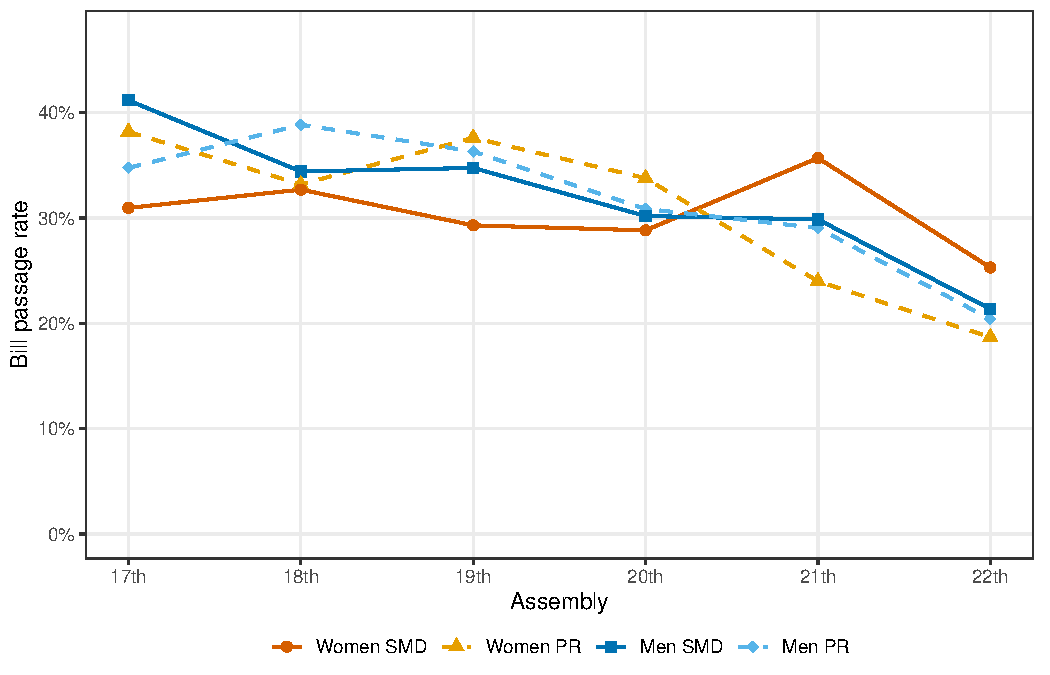
\includegraphics[width=\textwidth]{figures/2026-04-01_r6/fig_1.pdf}
\caption{Bill passage rates by gender and mandate type, 17th to 22nd Assemblies. The lines for women elected in districts and women elected through PR cross between the 20th and 21st Assemblies. Men's rates by mandate type differ by 6.4 and 4.4 points in the 17th and 18th Assemblies and by at most 1.6 points from the 19th on.}
\label{fig:passage}
\end{figure}

Figure~\ref{fig:passage} plots the same rates. Passage rates also fall for most groups across the recent Assemblies, which matters for the within-person comparison below.

\subsection{Pooled Regression Results}

\begin{table}[htbp]
\centering
\caption{Pooled Estimates, 20th to 22nd Assemblies: Bill Passage (Linear Probability Model)}
\label{tab:main}
\small
\begin{tabular}{lccccc}
\toprule
& (1) & (2) & (3) & (4) & (5) \\
& Baseline & + Assembly & + Party & + Seniority & + Committee \\
\midrule
Female               & $-0.014$ & $-0.014$ & $-0.013$ & $-0.013$ & $-0.015$ \\
                     & (0.021) & (0.019) & (0.018) & (0.018) & (0.017) \\[3pt]
SMD                  & $0.004$ & $0.003$ & $-0.034$ & $-0.048^{**}$ & $-0.052^{***}$ \\
                     & (0.017) & (0.016) & (0.022) & (0.022) & (0.019) \\[3pt]
Female $\times$ SMD  & $0.037$ & $0.043^{*}$ & $0.044^{**}$ & $0.040^{*}$ & $0.047^{**}$ \\
                     & (0.024) & (0.023) & (0.022) & (0.022) & (0.020) \\[3pt]
Multi-term &  &  &  & $0.026^{***}$ & $0.024^{***}$ \\
 &  &  &  & (0.008) & (0.008) \\
\midrule
$N$             & 61,209 & 61,209 & 61,209 & 61,209 & 61,103 \\
Legislators (clusters) & 660 & 660 & 660 & 660 & 660 \\
Assembly FE     & No & Yes & Yes & Yes & Yes \\
Party FE        & No & No & Yes & Yes & Yes \\
Committee FE    & No & No & No & No & Yes \\
$R^2$           & 0.001 & 0.008 & 0.011 & 0.011 & 0.056 \\
\bottomrule
\end{tabular}

\vspace{4pt}
\parbox{0.9\textwidth}{\footnotesize \textit{Note}: $^*p<0.10$, $^{**}p<0.05$, $^{***}p<0.01$. Standard errors clustered by lead sponsor in parentheses. Member bills of the 20th to 22nd Assemblies whose lead sponsor is in that Assembly's member file. Multi-term is 1 when the lead sponsor's term number at that Assembly is above 1 (Section~\ref{sec:seniority}). Column 5 drops 105 bills with no committee referral and one bill whose committee appears only once.}
\end{table}

Table~\ref{tab:main} reports the pooled model for the 20th through 22nd Assemblies. In the baseline, the district minus PR gap is 3.7 points larger for women than for men, an estimate not distinguishable from zero at the 10 percent level. With Assembly fixed effects the difference is 4.3 points, and with party fixed effects 4.4 points, distinguishable from zero at the 5 percent level. Adding the multi-term indicator in column 4 lowers the interaction to 4.0 points, a reduction of about 9 percent. With committee-referral fixed effects the interaction is 4.7 points. Bills of multi-term sponsors pass about 2.6 points more often than bills of first-term sponsors with the same gender, route, Assembly and party. The seniority indicator is therefore associated with passage, but it absorbs little of the pathway interaction, contrary to P3.

\subsection{Assembly-Specific Estimates}

\begin{table}[htbp]
\centering
\caption{Assembly-Specific Estimates: Bill Passage (Linear Probability Model)}
\label{tab:assembly}
\footnotesize
\begin{tabular}{lcccccc}
\toprule
& (1) & (2) & (3) & (4) & (5) & (6) \\
& 20th & 20th & 21st & 21st & 22nd & 22nd \\
& & + Seniority & & + Seniority & & + Seniority \\
\midrule
Female               & $0.023$ & $0.022$ & $-0.039$ & $-0.036$ & $-0.015$ & $-0.016$ \\
                     & (0.035) & (0.035) & (0.028) & (0.028) & (0.024) & (0.024) \\[3pt]
SMD                  & $-0.017$ & $-0.030$ & $-0.020$ & $-0.037$ & $0.060$ & $0.052$ \\
                     & (0.031) & (0.033) & (0.041) & (0.043) & (0.040) & (0.038) \\[3pt]
Female $\times$ SMD  & $-0.032$ & $-0.037$ & $0.100^{***}$ & $0.093^{**}$ & $0.055^{*}$ & $0.054^{*}$ \\
                     & (0.042) & (0.043) & (0.036) & (0.036) & (0.032) & (0.032) \\[3pt]
Multi-term &  & $0.021$ &  & $0.037^{***}$ &  & $0.017$ \\
 &  & (0.017) &  & (0.013) &  & (0.011) \\
\midrule
$N$         & 21,594 & 21,594 & 23,652 & 23,652 & 15,963 & 15,963 \\
Party FE    & Yes & Yes & Yes & Yes & Yes & Yes \\
$R^2$       & 0.002 & 0.003 & 0.007 & 0.008 & 0.005 & 0.005 \\
\bottomrule
\end{tabular}

\vspace{4pt}
\parbox{0.9\textwidth}{\footnotesize \textit{Note}: $^*p<0.10$, $^{**}p<0.05$, $^{***}p<0.01$. Standard errors clustered by lead sponsor in parentheses. Multi-term is seniority at that Assembly. In the 22nd Assembly the two codings of Table~\ref{tab:coding} coincide, because the member files end with it.}
\end{table}

Table~\ref{tab:assembly} estimates the model separately for each Assembly with party fixed effects. In the 20th Assembly the interaction is $-$3.2 points and not distinguishable from zero. In the 21st it is 10.0 points, distinguishable from zero at the 1 percent level, and in the 22nd it is 5.5 points, distinguishable from zero at the 10 percent level only. Adding seniority at the Assembly moves these estimates to $-$3.7, 9.3 and 5.4 points, reductions of about 7 percent in the 21st Assembly and 2 percent in the 22nd. Table~\ref{tab:coding} shows that the Version 1 coding would have produced 9.8 points for the 21st Assembly, so the halving that Version 1 reported does not appear under either coding.

\begin{figure}[htbp]
\centering
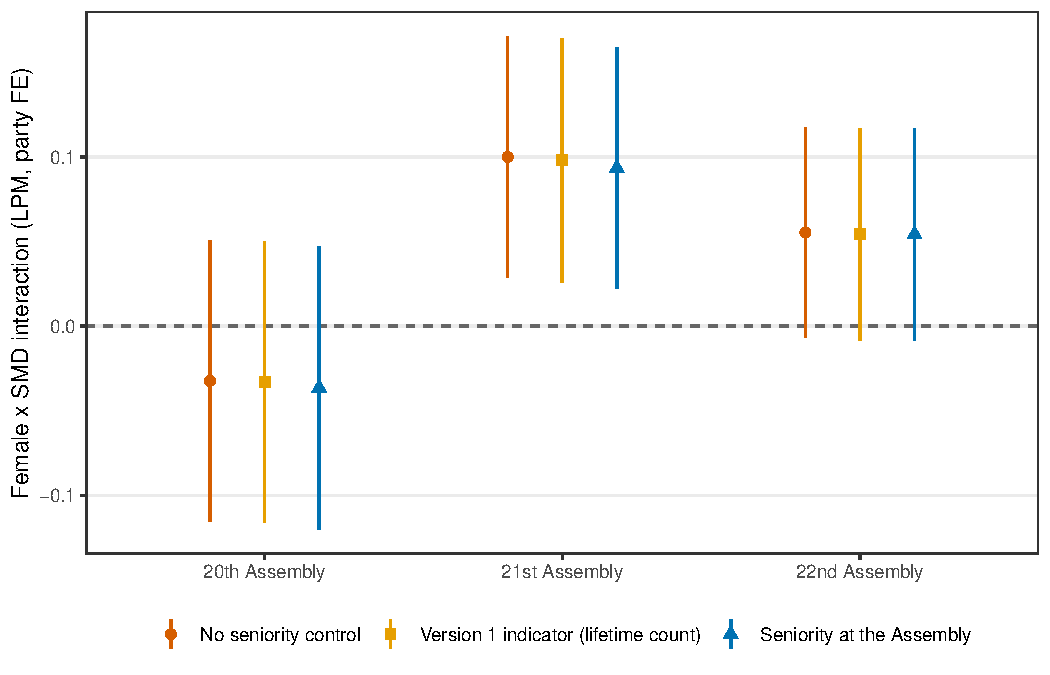
\includegraphics[width=\textwidth]{figures/2026-04-01_r6/fig_2.pdf}
\caption{Female $\times$ SMD interaction by Assembly, with party fixed effects and standard errors clustered by lead sponsor (Table~\ref{tab:assembly}), without a seniority control, with the Version 1 indicator based on the lifetime term count and with seniority at the Assembly. Bars show 95 percent intervals.}
\label{fig:coef}
\end{figure}

Figure~\ref{fig:coef} plots the three estimates for each Assembly. The sign change between the 20th and 21st Assemblies is visible under every specification, and neither seniority coding moves the estimates much.

\subsection{Seniority Composition}
\label{sec:composition}

\begin{table}[htbp]
\centering
\caption{Seniority at the Assembly and Passage Rates of Women Legislators, 20th to 22nd Assemblies}
\label{tab:composition}
\small
\begin{tabular}{p{0.52\textwidth}ccc}
\toprule
& 20th & 21st & 22nd \\
\midrule
\multicolumn{4}{l}{\textit{Panel A: Women legislators (member-terms)}} \\[3pt]
SMD women & 28 & 32 & 36 \\
\quad in a second or later term (\%) & 82 & 50 & 75 \\
PR women & 25 & 32 & 28 \\
\quad in a first term (\%) & 96 & 91 & 89 \\
\midrule
\multicolumn{4}{l}{\textit{Panel B: Passage rate of women's bills (\%), with bills and legislators}} \\[3pt]
SMD, second or later term & 28.1 & 36.7 & 25.1 \\
\quad bills, legislators & 1,903, 23 & 1,611, 16 & 1,761, 27 \\
SMD, first term & 31.7 & 33.9 & 25.9 \\
\quad bills, legislators & 505, 5 & 981, 16 & 552, 9 \\
PR, second or later term & 30.4 & 28.6 & 15.3 \\
\quad bills, legislators & 69, 1 & 35, 3 & 183, 3 \\
PR, first term & 33.9 & 23.9 & 19.2 \\
\quad bills, legislators & 1,974, 24 & 2,254, 29 & 1,300, 24 \\
\midrule
\multicolumn{4}{l}{\textit{Panel C: SMD minus PR among women (percentage points)}} \\[3pt]
All women & $-5.0$ & 11.7 & 6.6 \\
First-term women & $-2.2$ & 10.0 & 6.7 \\
All women, PR reweighted to the SMD seniority mix & $-2.3$ & 8.9 & 9.1 \\
\midrule
\multicolumn{4}{l}{\textit{Panel D: First-term women, bill-level LPM}} \\[3pt]
SMD & $-0.022$ & $0.100^{***}$ & $0.068^{**}$ \\
 & (0.037) & (0.033) & (0.033) \\
Number of bills & 2,479 & 3,235 & 1,852 \\
Number of legislators (clusters) & 29 & 45 & 33 \\
\bottomrule
\end{tabular}

\vspace{4pt}
\parbox{0.92\textwidth}{\footnotesize \textit{Note}: Seniority is the term number at that Assembly (Section~\ref{sec:seniority}). Panel C, last row: PR women's passage rates in the two seniority cells are weighted by the share of SMD women's bills sponsored by members in a second or later term, and the reweighted PR rate is subtracted from the SMD rate. Panel D regresses passage on an SMD indicator among bills of first-term women, with standard errors clustered by lead sponsor in parentheses. $^*p<0.10$, $^{**}p<0.05$, $^{***}p<0.01$.}
\end{table}

PR women were almost all in a first term. In the 20th, 21st and 22nd Assemblies, 96, 91 and 89 percent of PR women were serving their first term (Table~\ref{tab:composition} and Figure~\ref{fig:seniority}). District women were more senior, but not uniformly so. The share of district women in a second or later term was 82 percent in the 20th Assembly, 50 percent in the 21st and 75 percent in the 22nd. Version 1 reported 81 percent for the 21st Assembly, because its coding counted as experienced the ten district women who were in their first term in the 21st and were re-elected in 2024.

\begin{figure}[htbp]
\centering
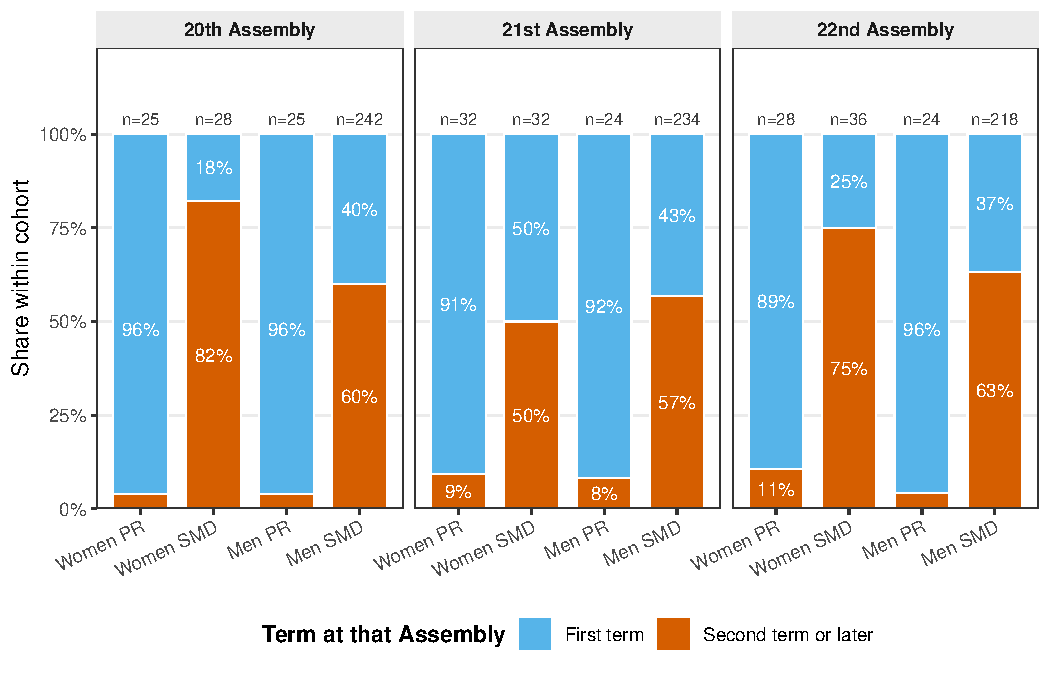
\includegraphics[width=\textwidth]{figures/2026-04-01_r6/fig_3.pdf}
\caption{Share of legislators in a first term and in a second or later term at that Assembly, by gender and mandate type, 20th to 22nd Assemblies. Seniority is the term number derived for each Assembly (Section~\ref{sec:seniority}). The Version 1 figure used the lifetime term count.}
\label{fig:seniority}
\end{figure}

This pattern runs against P1. The seniority gap between district and PR women was widest in the 20th Assembly, when PR women passed 5.0 points more of their bills, and narrowest in the 21st, when district women passed 11.7 points more.

Within seniority cells the gap persists. In the 21st Assembly, first-term district women passed 33.9 percent of their bills and first-term PR women 23.9 percent, a difference of 10.0 points against 11.7 points among all women. The comparison rests on 16 district women and 29 PR women, and the bill-level estimate in Panel D of Table~\ref{tab:composition} is distinguishable from zero at the 1 percent level. Only three PR women were beyond a first term in the 21st Assembly, so the comparison among experienced women carries little information. In the 22nd Assembly, first-term district women passed 6.7 points more than first-term PR women, against an aggregate gap of 6.6 points. In the 20th, first-term district women passed 2.2 points less, a comparison that rests on five district women.

Reweighting PR women's cell rates to the seniority mix of district women's bills leaves 8.9 of the 11.7-point gap in the 21st Assembly, so seniority composition accounts for about a quarter of it. In the 22nd Assembly the reweighting widens the gap from 6.6 to 9.1 points, because the three PR women beyond a first term passed fewer of their bills than first-term PR women. Under the Version 1 coding the same calculation accounts for 8 percent of the 21st Assembly gap, so Version 1's statement that composition alone could generate the reversal did not hold even under its own coding.

\subsection{Within-Party Comparison}

\begin{table}[htbp]
\centering
\caption{Passage Rates of Women by Mandate Type Within Party Blocs (\%)}
\label{tab:blocs}
\small
\begin{tabular}{llccccccc}
\toprule
& & \multicolumn{3}{c}{Passage rate} & \multicolumn{2}{c}{Bills} & \multicolumn{2}{c}{Legislators} \\
\cmidrule(lr){3-5}\cmidrule(lr){6-7}\cmidrule(lr){8-9}
Assembly & Bloc & SMD & PR & Gap & SMD & PR & SMD & PR \\
\midrule
20th & Progressive & 29.3 & 30.6 & $-1.3$ & 2,052 & 1,371 & 22 & 16 \\
20th & Conservative & 25.8 & 40.2 & $-14.4$ & 356 & 672 & 6 & 9 \\
21st & Progressive & 34.4 & 22.4 & 12.0 & 1,947 & 1,422 & 21 & 19 \\
21st & Conservative & 39.7 & 28.8 & 10.9 & 645 & 704 & 11 & 12 \\
22nd & Progressive & 25.0 & 17.6 & 7.4 & 1,700 & 908 & 24 & 17 \\
22nd & Conservative & 26.1 & 20.3 & 5.8 & 613 & 575 & 12 & 10 \\
\bottomrule
\end{tabular}

\vspace{4pt}
\parbox{0.92\textwidth}{\footnotesize \textit{Note}: Party labels from the member files. The bloc lists are those of Version 1 with the two proportional-list satellites of 2024, 국민의미래 and 더불어민주연합, added to the conservative and progressive blocs. Independents and parties outside both lists are left out.}
\end{table}

A difference in party composition between the two groups of women could produce the reversal. Table~\ref{tab:blocs} therefore compares district and PR women within the progressive and conservative blocs. In the 21st Assembly, district women passed more of their bills than PR women in both blocs, by 12.0 points among progressives and 10.9 points among conservatives. In the 22nd Assembly the differences are 7.4 and 5.8 points. In the 20th, PR women passed more in both blocs, by 1.3 and 14.4 points. The difference therefore appears on both sides of the partisan divide, which argues against an account based on one camp's majority status alone.\footnote{Version 1's lists place the 2020 party 국민의당 in the progressive bloc. Leaving its two women out lowers the 21st Assembly passage rate of progressive PR women from 22.4 to 21.6 percent.}

\subsection{Within-Person Comparison}

\begin{table}[htbp]
\centering
\caption{Passage Rates of Women Who Moved from a PR Seat to a District Seat}
\label{tab:switchers}
\small
\begin{tabular}{lcccccc}
\toprule
& Women & Negative & Mean (points) & 95\% interval & $t$ & $p$ \\
\midrule
\multicolumn{7}{l}{\textit{Raw change, first SMD term minus last PR term}} \\[3pt]
All pairs & 24 & 15 & $-5.6$ & $-11.6$ to 0.5 & $-1.90$ & 0.070 \\
Consecutive Assemblies only & 15 & 9 & $-2.8$ & $-10.7$ to 5.2 & $-0.75$ & 0.468 \\
\midrule
\multicolumn{7}{l}{\textit{Change net of the change among other PR women}} \\[3pt]
All pairs & 24 & 10 & $-1.3$ & $-8.5$ to 5.9 & $-0.37$ & 0.718 \\
Consecutive Assemblies only & 15 & 4 & 1.3 & $-7.1$ to 9.7 & 0.33 & 0.746 \\
\bottomrule
\end{tabular}

\vspace{4pt}
\parbox{0.95\textwidth}{\footnotesize \textit{Note}: One pair per woman, her last PR term and her first later SMD term, with passage rates over all bills she introduced as lead sponsor in each term. 15 of the 24 pairs are in consecutive Assemblies. The benchmark in the lower panel is the change in the passage rate of all other PR women between the same two Assemblies. Negative counts the women whose change is below zero. One-sample $t$-tests of the mean against zero.}
\end{table}

Twenty-four women held a PR seat and later a district seat. Table~\ref{tab:switchers} compares each woman's passage rate in her last PR term with that in her first later district term. Fifteen of the 24 passed a smaller share of their bills after the move, and the mean change is a decline of 5.6 points, which is not distinguishable from zero at the 5 percent level. Passage rates fell for most groups between Assemblies. Net of the change among other PR women between the same two Assemblies, the mean change is a decline of 1.3 points, with a 95 percent interval running from a decline of 8.5 points to a rise of 5.9 points, and 10 of the 24 women fall below zero. Nine of the 24 pairs skip at least one Assembly, and among the 15 consecutive pairs the net change is a rise of 1.3 points.

\begin{figure}[htbp]
\centering
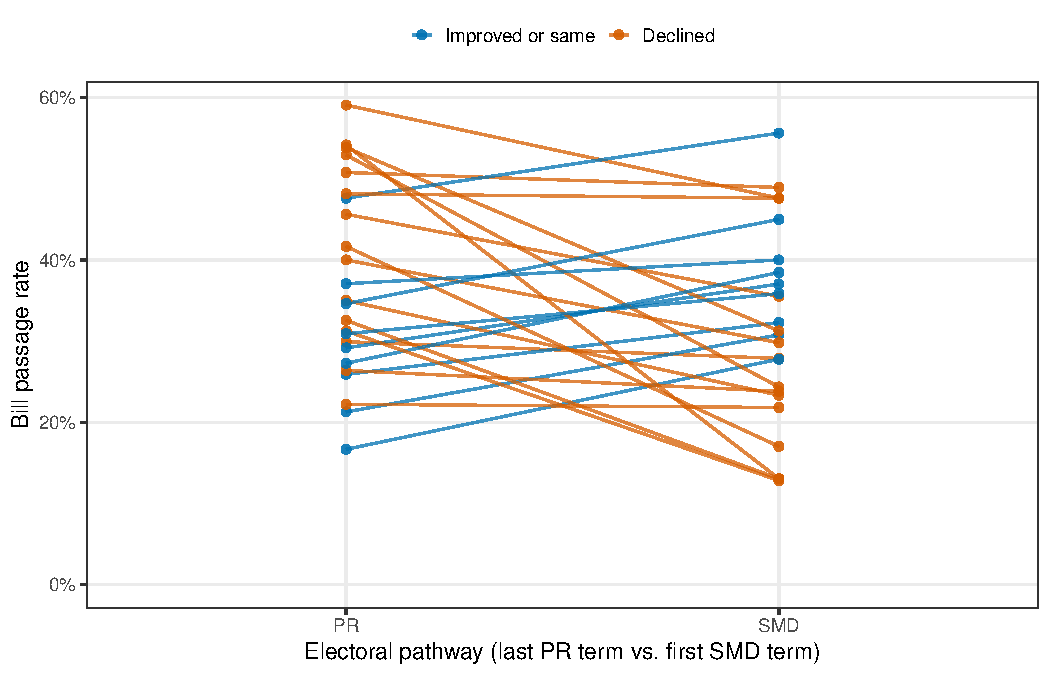
\includegraphics[width=\textwidth]{figures/2026-04-01_r6/fig_4.pdf}
\caption{Passage rates of 24 women in their last PR term and their first later district term. Fifteen of the 24 passed a smaller share of their bills after the move.}
\label{fig:switcher}
\end{figure}

All 24 women were in their second term when they first held a district seat, so the comparison changes seniority as well as the route. The data show neither the rise that the political capital account predicts nor a decline net of the trend, and the interval is too wide to rule out modest changes in either direction. The comparison therefore does not discriminate between P2 and the political capital account.

\subsection{Gender-Related Legislation}

Version 1 also reported a decline in gender-related bills that was steeper among PR women. With the four title keywords Version 1 lists, 성평등, 여성, 양성평등 and 성차별, such bills are rare. Their share of member bills was 0.26 percent in the 19th Assembly, 0.25 percent in the 20th, 0.22 percent in the 21st and 0.20 percent in the 22nd. The same keywords in the proposal-reason texts, available from the 20th Assembly on, match 4.1, 2.7 and 2.3 percent of bills in the 20th, 21st and 22nd. Among women, the title-keyword share of PR members was at least as high as that of district members in each of these three Assemblies, and each cell holds between 6 and 16 bills. These counts do not support Version 1's reading that party gatekeeping restrained PR women's gender-related legislation, and that reading is withdrawn. The decline in the proposal-reason measure is compatible with the backlash that \citet{woo2023} document for bills on violence against women, but this paper does not test that link.

\subsection{Robustness}
\label{sec:robustness}

\begin{table}[htbp]
\centering
\caption{Robustness: Comparable Windows and Direct Enactment}
\label{tab:robust}
\small
\begin{tabular}{p{0.5\textwidth}ccc}
\toprule
& 20th & 21st & 22nd \\
\midrule
\multicolumn{4}{l}{\textit{Panel A: Bills introduced in the first ten months (passage rate, \%)}} \\[3pt]
Women, SMD & 31.1 & 41.5 & 33.7 \\
Women, PR & 46.4 & 32.5 & 29.3 \\
Women, SMD minus PR (points) & $-15.3$ & 9.0 & 4.4 \\
Men, SMD minus PR (points) & 2.3 & 1.1 & 0.1 \\
Bills in the window & 5,663 & 8,374 & 8,552 \\
\midrule
\multicolumn{4}{l}{\textit{Panel B: Direct enactment only (rate, \%)}} \\[3pt]
Women, SMD & 4.7 & 7.2 & 2.9 \\
Women, PR & 6.9 & 3.4 & 3.0 \\
Women, SMD minus PR (points) & $-2.2$ & 3.8 & $-0.1$ \\
\midrule
\multicolumn{4}{l}{\textit{Panel C: Direct enactment, pooled LPM, Female $\times$ SMD}} \\[3pt]
Table~\ref{tab:main}, column 3 specification & \multicolumn{3}{c}{$0.008$ (0.009)} \\
Adding the multi-term indicator & \multicolumn{3}{c}{$0.007$ (0.010)} \\
$N$ & \multicolumn{3}{c}{61,209} \\
\bottomrule
\end{tabular}

\vspace{4pt}
\parbox{0.92\textwidth}{\footnotesize \textit{Note}: Panel A keeps bills introduced from 30 May of the Assembly's first year through the day before the ten-month mark. Panel B counts only bills passed in their original or amended form, leaving out bills absorbed into a committee alternative. Panel C, standard errors clustered by lead sponsor in parentheses, with assembly and party fixed effects. $^*p<0.10$, $^{**}p<0.05$, $^{***}p<0.01$.}
\end{table}

\textit{Co-sponsorship.} Mean co-sponsor counts per bill range from 11.4 to 12.0 across the four gender and mandate cells of the 20th through 22nd Assemblies, so differences in coalition size are unlikely to account for the gap.

\textit{Comparable windows.} Restricting each Assembly to bills introduced in its first ten months, PR women passed 15.3 points more of their bills than district women in the 20th Assembly, and district women passed 9.0 points more in the 21st and 4.4 points more in the 22nd (Table~\ref{tab:robust}). Among men the district minus PR difference is at most 2.3 points in these windows. The reversal is therefore not a product of the 22nd Assembly's shorter observation period.

\textit{Direct enactment.} Counting only bills passed in their original or amended form, district women passed 7.2 percent of their bills in the 21st Assembly and PR women 3.4 percent, a difference of 3.8 points against 11.7 points under the main definition. In the 22nd Assembly the two rates are 2.9 and 3.0 percent, and in the 20th PR women lead by 2.2 points. In the pooled model the interaction is 0.8 points and not distinguishable from zero, and adding the seniority indicator leaves it at 0.7 points. Much of the reversal, and all of it in the 22nd Assembly, therefore lies in bills absorbed into committee alternatives.

\begin{table}[htbp]
\centering
\caption{Seniority Estimates in Version 1 and Reruns Under Two Codings}
\label{tab:coding}
\small
\begin{tabular}{p{0.40\textwidth}ccc}
\toprule
& Version 1 & \multicolumn{2}{c}{Rerun on the pinned data} \\
\cmidrule(lr){3-4}
& published & Lifetime count & Term at the Assembly \\
\midrule
Pooled, column 4: Female $\times$ SMD & $0.019$ & $0.044^{**}$ & $0.040^{*}$ \\
 & (0.018) & (0.022) & (0.022) \\[2pt]
Pooled, column 4: Multi-term & $0.068$ & $0.014$ & $0.026^{***}$ \\
 & (0.012) & (0.009) & (0.008) \\[2pt]
Pooled, column 5: Female $\times$ SMD & $0.015$ & $0.051^{**}$ & $0.047^{**}$ \\
 & (0.019) & (0.020) & (0.020) \\[2pt]
Pooled, column 5: Multi-term & $0.059$ & $0.014^{*}$ & $0.024^{***}$ \\
 & (0.012) & (0.008) & (0.008) \\[2pt]
20th, with seniority: Female $\times$ SMD & $-0.021$ & $-0.033$ & $-0.037$ \\
 & (0.031) & (0.042) & (0.043) \\[2pt]
21st, with seniority: Female $\times$ SMD & $0.058$ & $0.098^{***}$ & $0.093^{**}$ \\
 & (0.029) & (0.037) & (0.036) \\[2pt]
22nd, with seniority: Female $\times$ SMD & $0.027$ & $0.054^{*}$ & $0.054^{*}$ \\
 & (0.034) & (0.032) & (0.032) \\[2pt]
20th: Multi-term & $0.062$ & $-0.003$ & $0.021$ \\
 & (0.014) & (0.019) & (0.017) \\[2pt]
21st: Multi-term & $0.071$ & $0.020$ & $0.037^{***}$ \\
 & (0.014) & (0.014) & (0.013) \\[2pt]
22nd: Multi-term & $0.058$ & $0.017$ & $0.017$ \\
 & (0.017) & (0.011) & (0.011) \\[2pt]
\bottomrule
\end{tabular}

\vspace{4pt}
\parbox{0.92\textwidth}{\footnotesize \textit{Note}: Lifetime count is the Version 1 coding, multi-term when the member file's \texttt{reelection} field is not 초선. Term at the Assembly is the Version 2 coding. Specifications of Tables~\ref{tab:main} and~\ref{tab:assembly}, standard errors clustered by lead sponsor in parentheses. Stars are shown for the reruns only, $^*p<0.10$, $^{**}p<0.05$, $^{***}p<0.01$.}
\end{table}


%% ============================================================
%%  5. DISCUSSION
%% ============================================================
\section{Discussion}

The corrected analysis separates two claims that Version 1 joined. The first is descriptive. In the 21st and 22nd Assemblies, women elected in districts passed a larger share of their bills than women elected through PR, after the opposite pattern in the 17th through 20th, and the difference appears within both party blocs and in comparable ten-month windows. The second is explanatory, and it does not hold. Seniority at the Assembly is associated with passage, and PR women are almost all newcomers, but seniority composition accounts for about a quarter of the 21st Assembly gap and none of the 22nd, in the 21st and 22nd Assemblies the gap is about as large among first-term women as among all women, and the seniority gap between the two groups of women was widest in the Assembly in which PR women passed more.

The within-person comparison is uninformative about the source of the reversal. Women who moved to a district seat passed fewer of their bills afterward, but no more than the fall among other PR women, and the move coincided with each woman's second term. The comparison neither shows that winning a district brings leverage nor shows that it does not.

What the reversal reflects is therefore an open question. Several possibilities are consistent with the data, and none is tested here. In the 2020 election both major parties ran proportional-list satellite parties, and 18 of the 32 PR women of the 21st Assembly carry a satellite label in the member file, although the same holds for 18 of the 28 PR women of the 22nd. Committee alignment, which \citet{an2025} associate with passage, is unmeasured, and the committee-referral fixed effects, which leave the interaction slightly larger, do not capture it. The reversal is concentrated in absorption into committee alternatives, especially in the 22nd Assembly, so how committee chairs consolidate related bills may matter. Survivor selection also complicates any seniority comparison, because district women beyond a first term are the ones voters re-elected.

Several limitations bound the analysis. First, the design is observational, and no estimate is a causal effect of the electoral route or of seniority. Second, the multi-term indicator is coarse and does not measure committee tenure or leadership positions. Third, the 22nd Assembly is incomplete, with most of its bills still pending. Fourth, the within-person comparison covers 24 women and changes seniority together with the route. Fifth, the bloc classification relies on party labels recorded at the start of each term. Sixth, the hypothesis was formulated after the reversal had been observed.

The error that Version 1 made has a general lesson for work with legislative member files. A seniority field recorded at collection describes a member's whole career, and reading it as seniority at an earlier Assembly sorts members by whether they were later re-elected.


%% ============================================================
%%  6. CONCLUSION
%% ============================================================
\section{Conclusion}

Women elected in single-member districts of the Korean National Assembly passed a larger share of their bills than women elected through proportional representation in the 21st and 22nd Assemblies, reversing the pattern of the 17th through 20th. Version 1 of this paper attributed the reversal to a seniority asymmetry created by the PR gender quota. With seniority measured at each Assembly, that explanation accounts for little of the reversal. Adding a multi-term indicator changes the pathway interaction by about a tenth, the gap persists among first-term women, and the seniority gap between district and PR women was widest when PR women passed more. The within-person comparison of women who moved from PR to district seats does not distinguish among the explanations.

Future research could address the questions left open. Committee membership data for all Assemblies would allow a test of committee alignment. A study of how committee alternatives absorb bills would show why the reversal runs mainly through that channel. Following the cohorts of the 21st and 22nd Assemblies would show whether the reversal outlasts the satellite-party elections of 2020 and 2024.


\bigskip
\noindent\textbf{AI-generation disclosure.} This working paper was generated by AI research agents (kna-research-agents.com) as an experimental output. Version 2 was corrected by the orchestrating Claude session at the researcher's request after an audit of the seniority coding, as the correction notice describes. No human author of record exists, and the authorship line denotes the agent system. The paper has not been peer-reviewed or independently fact-checked. Do not cite or use it in any academic, policy, or professional context.

\medskip
\noindent\textbf{Data availability.} All analyses use the processed files of the Korean National Assembly legislative database (github.com/kyusik-yang/kna) at release v0.6.0, commit 4e28c1e. Its member and bill files are the same as in the release that Version 1 used. The derived term numbers were checked against the \texttt{term\_number} field of release v0.7.1. The figure scripts in the paper's figures folder read the pinned files through the \texttt{KNA\_DATA\_V060} environment variable and regenerate Figures~\ref{fig:passage} to~\ref{fig:switcher}. The table values were computed by a rerun script in the project's working files, which is not published with this paper.

\bibliographystyle{apsr}
\bibliography{references_r6}

\end{document}
